\documentclass[11pt]{article}
\usepackage[utf8]{inputenc}
\usepackage[T1]{fontenc}
\usepackage[spanish]{babel}
\usepackage{amsmath, amssymb}
\usepackage{graphicx}
\usepackage{float}
\usepackage[margin=2.5cm]{geometry}

\title{Business Intelligence\\Tarea 4: Introducci\'on a Series de Tiempo}
\author{Noel Eduardo Sánchez Useda}
\date{25 de octubre de 2026}

\begin{document}
\maketitle

\section*{Parte 0: Procesos simulados}

\subsection*{0.1 Derivaciones a mano}

Sea el AR(1) estacionario $Y_t = c + \phi Y_{t-1} + \varepsilon_t$, con
$|\phi|<1$ y $\varepsilon_t \overset{\text{iid}}{\sim} \mathcal{N}(0,\sigma^2)$.

\paragraph{Media.} Por estacionariedad, $E[Y_t]=E[Y_{t-1}]=\mu$. Tomando
esperanza en ambos lados:
\[
\mu = c + \phi\mu + 0 \;\Longrightarrow\; \mu(1-\phi)=c
\;\Longrightarrow\; E[Y_t]=\frac{c}{1-\phi}.
\]

\paragraph{Varianza.} Como $\varepsilon_t$ es independiente de $Y_{t-1}$ y
$\mathrm{Var}(Y_t)=\mathrm{Var}(Y_{t-1})=\gamma_0$:
\[
\gamma_0 = \phi^2\gamma_0 + \sigma^2
\;\Longrightarrow\; \gamma_0(1-\phi^2)=\sigma^2
\;\Longrightarrow\; \mathrm{Var}(Y_t)=\frac{\sigma^2}{1-\phi^2}.
\]
Se necesita $|\phi|<1$ para que el denominador sea estrictamente positivo; si
$\phi=1$ la expresi\'on no est\'a definida y no existe una varianza
estacionaria finita.

\paragraph{Autocorrelaci\'on.} Como $c=\mu(1-\phi)$, el proceso centrado es
$Y_t-\mu=\phi(Y_{t-1}-\mu)+\varepsilon_t$. Multiplicando por $(Y_{t-k}-\mu)$
con $k\ge 1$ y tomando esperanza:
\[
\gamma_k = \phi\,\gamma_{k-1} + E[\varepsilon_t(Y_{t-k}-\mu)] = \phi\,\gamma_{k-1},
\]
pues $\varepsilon_t$ es independiente de todo el pasado. Aplicando la
recursi\'on $k$ veces, $\gamma_k=\phi^k\gamma_0$, y por tanto
\[
\rho_k=\frac{\gamma_k}{\gamma_0}=\phi^k.
\]

\paragraph{Caminata aleatoria} ($\phi=1$, $c=0$, $Y_0=0$). Sustituyendo hacia
atr\'as, $Y_t=\sum_{i=1}^{t}\varepsilon_i$, as\'i que
\[
\mathrm{Var}(Y_t)=\sum_{i=1}^{t}\mathrm{Var}(\varepsilon_i)=t\sigma^2 .
\]
La estacionariedad d\'ebil exige varianza constante en el tiempo. Aqu\'i
$\mathrm{Var}(Y_1)=\sigma^2$, $\mathrm{Var}(Y_2)=2\sigma^2,\dots$, es decir,
crece linealmente con $t$, por lo que el proceso no es estacionario.

\subsection*{0.2 Simulaci\'on}

\paragraph{Por qu\'e se descartan los primeros 200 pasos.} Para $|\phi|<1$, la
influencia del valor inicial decae como $\phi^t$, de modo que al llegar a
$t=200$ el proceso ya olvid\'o $Y_0$ y su varianza se estabiliz\'o en
$\sigma^2/(1-\phi^2)$. Para $\phi=1$ eso no ocurre: la memoria de $Y_0$ nunca
decae y $\mathrm{Var}(Y_t)=t\sigma^2$ sigue creciendo, as\'i que no existe un
estado estacionario al cual converger.

\paragraph{Por qu\'e el descarte no afecta a $r_k$ cuando $\phi=1$.} Si se
descartan los primeros 200 pasos, el tramo restante es
$Y_t = Y_{200} + \sum_{i=201}^{t}\varepsilon_i$. La autocorrelaci\'on muestral
$r_k$ usa las desviaciones $y_t-\bar{y}$, y la constante $Y_{200}$ se cancela
al restar la media muestral. Lo que queda es una caminata aleatoria que
parte de cero con incrementos iid, cuya distribuci\'on es la misma que la de
la serie completa. Por eso el punto de partida no altera la distribuci\'on de
$r_k$.

\paragraph{Resultados (5{,}000 r\'eplicas por $\phi$, $n=300$).}
La Figura~\ref{fig:real} muestra una realizaci\'on por escenario y el
Cuadro~\ref{tab:p02} resume las r\'eplicas. Las semillas son
\texttt{SEED\_BASE}$+i$ para el escenario $i$, con \texttt{SEED\_BASE}$=2026$
(las realizaciones de la figura usan \texttt{SEED\_BASE}$+100+i$). El error
est\'andar de cada promedio es la desviaci\'on est\'andar entre
$\sqrt{5000}$; el de la tasa de rechazo $p$ es $\sqrt{p(1-p)/5000}$.

\begin{figure}[H]
\centering
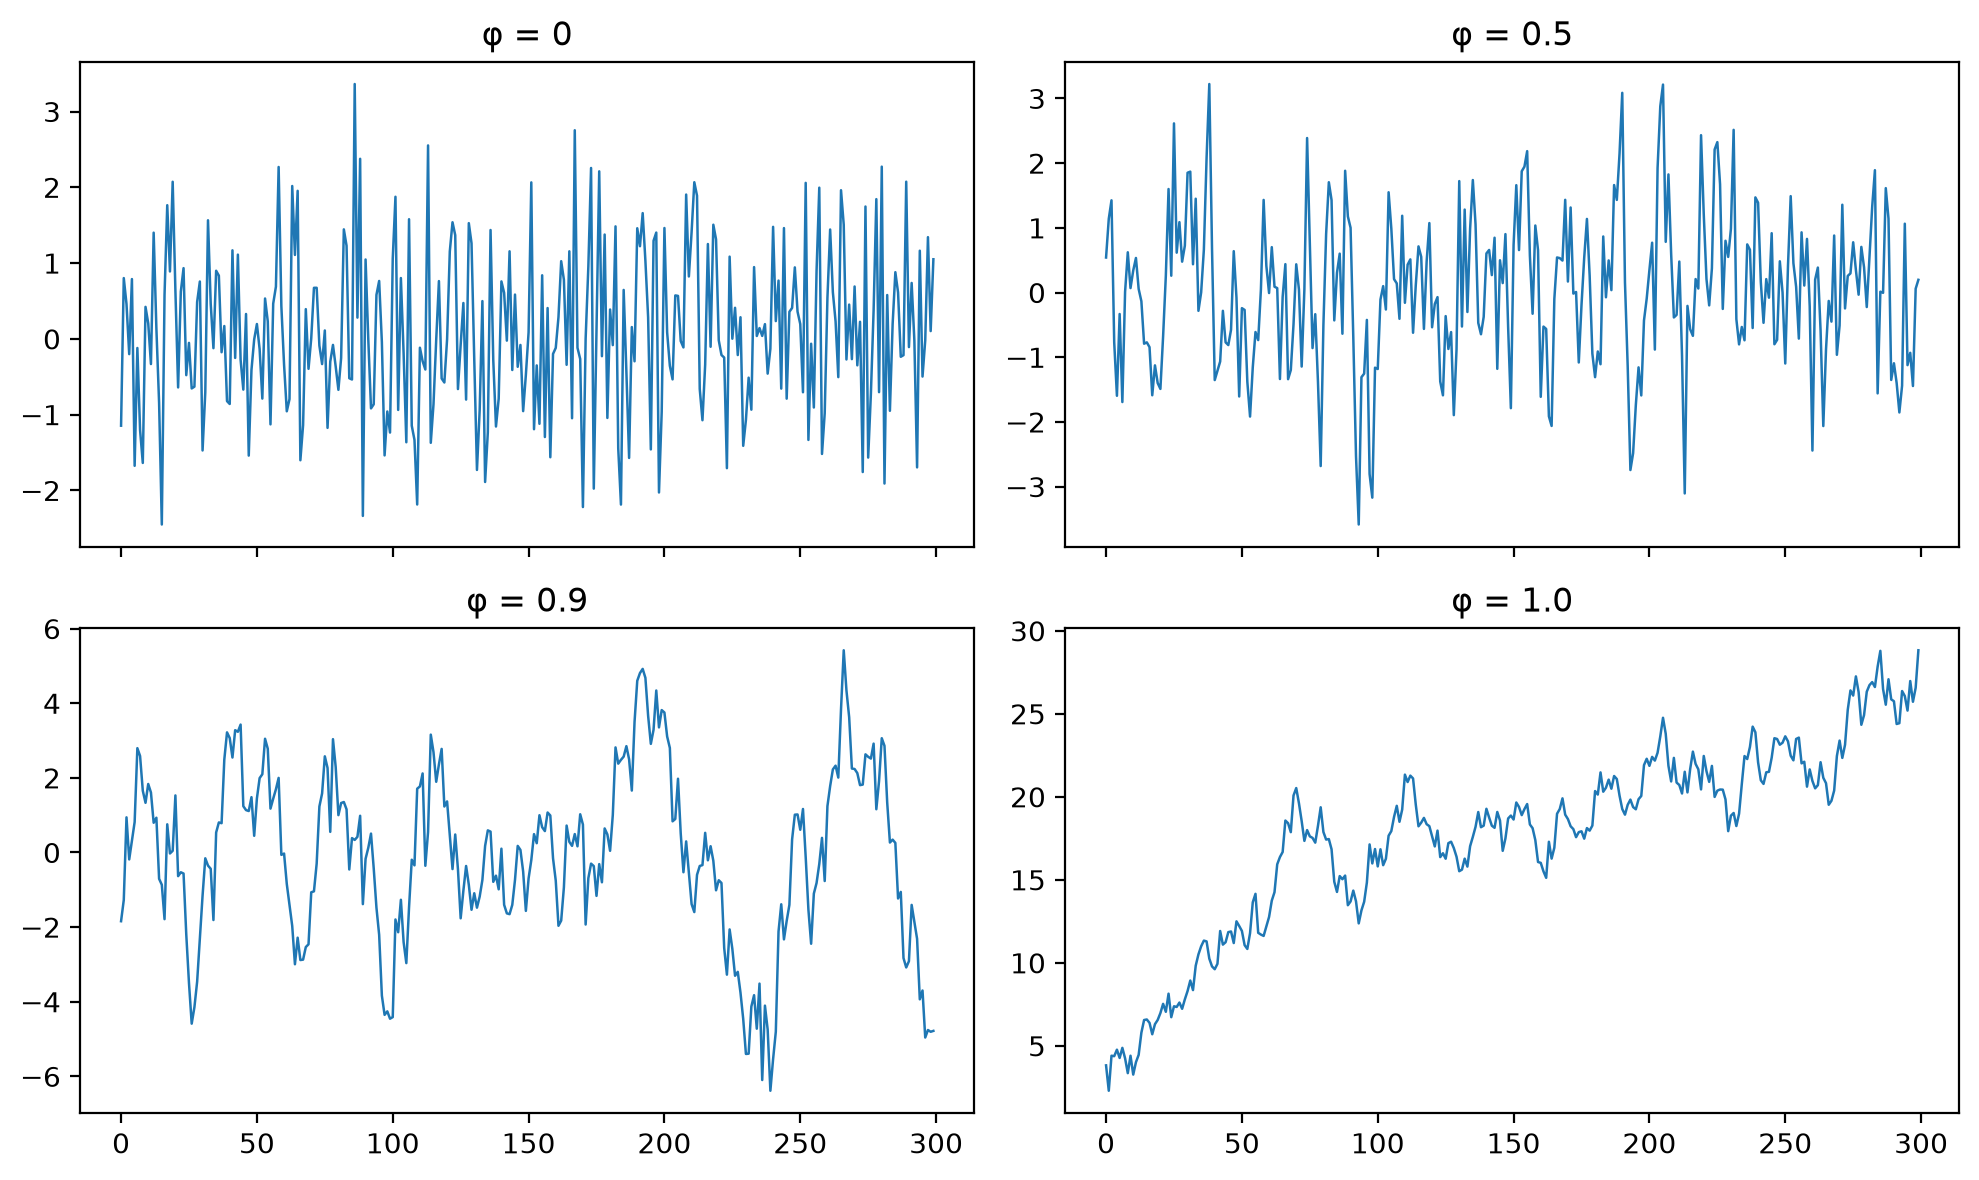
\includegraphics[width=0.85\textwidth]{p0_realizaciones.png}
\caption{Una realizaci\'on de 300 pasos por $\phi\in\{0,0.5,0.9,1\}$. Con
$\phi=0$ la serie oscila r\'apidamente alrededor de 0 sin patr\'on visible
(ruido blanco). Al aumentar $\phi$ los valores cercanos se parecen m\'as y
aparecen tramos largos del mismo lado de la media, m\'as largos con
$\phi=0.9$. Con $\phi=1$ la serie vaga a la deriva sin regresar a un nivel de
equilibrio, lo que refleja $\mathrm{Var}(Y_t)=t\sigma^2$. La tendencia
ascendente que se ve en esta realizaci\'on es producto del azar, no una
tendencia determinista.}
\label{fig:real}
\end{figure}

\begin{table}[H]
\centering
\resizebox{\textwidth}{!}{%
\begin{tabular}{c|cc|cc|c|cc|cc}
\hline
$\phi$ & $\bar r_1$ & e.e. & $\bar r_5$ & e.e. & $\phi^5$ &
rechazo $r_1$ & e.e. & $\bar{\hat\phi}_{OLS}$ & e.e. \\
\hline
0.0 & $-0.0039$ & 0.0008 & $-0.0028$ & 0.0008 & 0.0000 & 0.0500 & 0.0031 & $-0.0039$ & 0.0008 \\
0.5 &  0.4892   & 0.0007 &  0.0199   & 0.0010 & 0.0312 & 1.0000 & 0.0000 &  0.4909   & 0.0007 \\
0.9 &  0.8839   & 0.0004 &  0.5339   & 0.0014 & 0.5905 & 1.0000 & 0.0000 &  0.8871   & 0.0004 \\
1.0 &  0.9758   & 0.0002 &  0.8835   & 0.0009 & 1.0000 & 1.0000 & 0.0000 &  0.9824   & 0.0002 \\
\hline
\end{tabular}}
\caption{Promedios sobre 5{,}000 r\'eplicas con su error est\'andar, tasa de
rechazo de la prueba $|r_1|>1.96/\sqrt{n}$ y promedio del estimado OLS de
$\phi$.}
\label{tab:p02}
\end{table}

\subsection*{0.3 An\'alisis}

\paragraph{Tasa de rechazo con $\phi=0$.} Es $0.0500$ (e.e.\ $0.0031$), que es
lo esperado. Con ruido blanco la hip\'otesis nula es cierta, y las bandas
$\pm1.96/\sqrt{n}$ corresponden a un nivel de significancia del 5\%. Como cada
r\'eplica produce un solo $r_1$, el 5\% de las \emph{r\'eplicas} cae fuera de
las bandas por puro azar.

\paragraph{Caminata aleatoria.} Para $\phi=1$ la teor\'ia da $\phi^5=1$, pero
el promedio de $r_5$ es 0.8835: la autocorrelaci\'on muestral queda por debajo
del valor te\'orico. La brecha respecto a $\phi^5$ crece al acercarse $\phi$ a 1
(0.0113 para $\phi=0.5$, 0.0566 para $\phi=0.9$ y 0.1165 para $\phi=1$), de
modo que en muestras finitas $r_k$ subestima $\phi^k$, y m\'as cuanto m\'as
persistente es la serie. Esto ocurre porque $r_k$ resta la media muestral
$\bar y$, estimada con los mismos datos: en una serie persistente $\bar y$
absorbe parte de la variaci\'on lenta, lo que reduce las desviaciones y
sesga $r_k$ hacia abajo. Adem\'as, el numerador suma $n-k$ t\'erminos mientras
el denominador suma $n$, lo que tambi\'en encoge $r_k$.

\paragraph{Sesgo del estimador OLS.} El promedio de $\hat\phi$ queda siempre
por debajo del $\phi$ verdadero y la diferencia mide varios errores
est\'andar, por lo que no es ruido de simulaci\'on. El sesgo es
$-0.0039$ para $\phi=0$, $-0.0091$ para $\phi=0.5$, $-0.0129$ para
$\phi=0.9$ y $-0.0176$ para $\phi=1$: se agudiza al acercarse a la ra\'iz
unitaria. Es un sesgo de muestra finita, del orden de $1/n$, que se reduce al
crecer $n$; por tanto el estimador OLS es consistente.

\subsection*{0.4 Las dos razones para reprobar}

\begin{table}[H]
\centering
\resizebox{\textwidth}{!}{%
\begin{tabular}{l|cc|cc|cc}
\hline
Proceso & $\bar r_1$ & e.e. & rechazo $r_1$ & e.e. & $\bar r_7$ & e.e. \\
\hline
$\phi=0$ (referencia) & $-0.0039$ & 0.0008 & 0.0500 & 0.0031 & $-0.0017$ & 0.0008 \\
(a) tendencia lineal  &  0.2446   & 0.0008 & 0.9834 & 0.0018 &  0.2297   & 0.0008 \\
(b) patr\'on semanal  & $-0.0476$ & 0.0007 & 0.1050 & 0.0043 &  0.2642   & 0.0008 \\
\hline
\end{tabular}}
\caption{Procesos sin memoria $Y_t=m_t+\varepsilon_t$ con 5{,}000 r\'eplicas
($n=300$). Semillas: \texttt{SEED\_BASE}$+0$ para $\phi=0$,
\texttt{SEED\_BASE}$+10$ para (a) y \texttt{SEED\_BASE}$+11$ para (b).}
\label{tab:p04}
\end{table}

\paragraph{(a) reprueba aunque no tiene memoria.} Los errores son
independientes, pero la media cambia con el tiempo: los primeros puntos quedan
por debajo de $\bar y$ y los \'ultimos por encima, de modo que las desviaciones
vecinas comparten signo, lo que infla $r_1$ ($\bar r_1=0.2446$) y produce una
tasa de rechazo de 98.34\%. Es la raz\'on (2) de la tarea: la media no es
constante. Por la misma raz\'on $\bar r_7=0.2297$ tambi\'en es positivo: la
tendencia infla las autocorrelaciones en todos los rezagos.

\paragraph{(b) casi pasa aunque tiene estructura.} La media del patr\'on es
exactamente 0. Para la mayor\'ia de los d\'ias consecutivos el producto es
$0.25\times0.25$, un valor positivo peque\~no, pero el d\'ia de $-1.5$ aparece
una vez por semana y participa en dos productos (con el d\'ia anterior y el
siguiente), cada uno de $-0.375$. Esos productos dominan la suma y empujan el
valor esperado de $r_1$ hacia valores negativos ($\bar r_1=-0.0476$), por lo
que la tasa de rechazo es 10.5\%: por encima del 5\% de la referencia, pero
muy por debajo de la de (a). La estructura aparece en el retardo 7, donde
$\bar r_7=0.2642$. Es moderado y no cercano a 1 porque el ruido ($\sigma^2=1$)
diluye la se\~nal: el valor aproximado es
$\mathrm{Var}(m)/(\mathrm{Var}(m)+\sigma^2)=0.375/1.375\approx0.27$.

\paragraph{Conexi\'on con RANDU.} Como RANDU, el patr\'on semanal parece
aleatorio e independiente si se mira con el lente equivocado. En RANDU basta
mirar los valores de uno en uno para que parezcan uniformes, y la estructura
aparece al graficar ternas consecutivas en tres dimensiones. En el patr\'on
semanal, mirar solo el retardo 1 oculta casi toda la estructura, que aparece
en el retardo 7. En ambos casos, una prueba que mira en la dimensi\'on
incorrecta no detecta la dependencia.

\subsection*{0.5 La prueba que s\'i ve}

\begin{table}[H]
\centering
\begin{tabular}{l|c|c|c}
\hline
Proceso & LB $m=10$ & LB $m=6$ & retardo 1 \\
\hline
$\phi=0$ (ruido blanco) & 0.0612 & 0.0600 & 0.0500 \\
(a) tendencia lineal    & 1.0000 & 1.0000 & 0.9834 \\
(b) patr\'on semanal    & 0.9514 & 0.1948 & 0.1050 \\
\hline
\end{tabular}
\caption{Tasa de rechazo al 5\% de Ljung--Box con $m=10$ y
$m=\mathrm{round}(\ln n)=6$, comparada con la prueba de retardo 1 (5{,}000
r\'eplicas, $n=300$). La implementaci\'on propia de $Q(10)$ coincide con
\texttt{acorr\_ljungbox} de \texttt{statsmodels}: en una serie de (b) ambas
dan $Q=61.0555$.}
\label{tab:p05}
\end{table}

Con ruido blanco, Ljung--Box rechaza el 6.12\% de las r\'eplicas ($m=10$) y el
6.00\% ($m=6$), cercano al 5\% esperado (con $n=300$ la prueba tiene un nivel
real ligeramente superior al nominal, adem\'as del ruido de simulaci\'on de
$\pm0.003$). En (a) rechaza siempre, igual que la prueba de retardo 1, por la
misma raz\'on: la media no es constante.

El cambio importante est\'a en (b): con $m=10$ la tasa de rechazo pasa de
10.5\% (retardo 1) a 95.1\%. La prueba de retardo 1 solo mira $r_1$, que en el
patr\'on semanal es peque\~no y negativo, as\'i que no ve el ciclo. $Q(10)$
suma $r_k^2/(n-k)$ para $k=1,\dots,10$ e incluye el retardo 7, donde
$\bar r_7=0.2642$. Su aporte a $Q$ es
\[
n(n+2)\frac{r_7^2}{n-7}=300\cdot302\cdot\frac{0.2642^2}{293}\approx 21.6,
\]
que por s\'i solo supera el valor cr\'itico de una $\chi^2_{10}$ al 5\%
($\approx 18.3$). Como todos los t\'erminos de la suma son no negativos,
$Q(10)\ge 21.6$ y el rechazo es casi seguro. Elevar $r_k$ al cuadrado evita
que las autocorrelaciones positivas y negativas se cancelen.

Con $m=6$ la tasa de (b) baja a 19.5\%, porque $Q(6)$ ya no incluye el retardo
7: solo acumula los rezagos 1 a 6, que tienen autocorrelaciones peque\~nas y
negativas inducidas por el patr\'on. Esto confirma que el rechazo de 95\% con
$m=10$ proviene del retardo 7, y que la elecci\'on de $m$ importa: una
ventana que no llega al ciclo no lo detecta bien. Por eso se recomienda
$m=2s$ cuando hay estacionalidad de periodo $s$.

En resumen, la prueba de un solo retardo tiene visi\'on de t\'unel y solo
detecta memoria inmediata. Revisar muchos rezagos por separado contra sus
bandas inflar\'ia los falsos positivos por comparaciones m\'ultiples; la
prueba portmanteau combina los primeros $m$ rezagos en un solo estad\'istico
con un nivel de significancia global del 5\%, y por eso detecta la estructura
semanal que el retardo 1 no ve.

\section*{Parte 1: Limpieza}

\subsection*{1.1 Carga de datos}

Los datos tienen 541{,}909 filas, 25{,}900 facturas, 4{,}070 c\'odigos de
producto (\texttt{StockCode}) y 4{,}372 clientes. El 24.93\% de las filas no
tiene \texttt{CustomerID}.

Las columnas \texttt{InvoiceNo}, \texttt{StockCode} y \texttt{CustomerID} se
leen como texto porque son identificadores, no cantidades: \texttt{InvoiceNo}
incluye prefijos con letras (\texttt{C} para cancelaciones y \texttt{A} para
ajustes contables), \texttt{StockCode} mezcla c\'odigos num\'ericos con letras
(\texttt{85123A}, \texttt{POST}) y \texttt{CustomerID}, al tener valores
faltantes, se leer\'ia como n\'umero decimal (\texttt{17850.0}) y dejar\'ia de
ser un identificador exacto.

\subsection*{1.2 Decisiones de limpieza}

Las letras de esta secci\'on describen las decisiones; las letras del
Cuadro~\ref{tab:bitacora} numeran las reglas en el orden en que se aplicaron.
La regla (c) de la bit\'acora (ventas anuladas por una cancelaci\'on manual) se
explica en 1.4.

\paragraph{(a) Filas duplicadas exactas: se eliminan.} Son 5{,}268 filas
id\'enticas en factura, producto, cantidad, hora, precio y cliente. Se asume que
son registros repetidos y no compras genuinas; conservarlas inflar\'ia la venta
(\pounds 21{,}740.98). Es un supuesto, pues no es posible descartar que alg\'un
art\'iculo se haya escaneado dos veces de verdad.

\paragraph{(b) Facturas que no empiezan con d\'igito.} Las que empiezan con
\texttt{C} (9{,}288 filas) \emph{se quedan}: son cancelaciones y su cantidad
negativa ya resta de la venta del d\'ia en que ocurren. Las que empiezan con
\texttt{A} (3 filas) \emph{se eliminan}: corresponden a ajustes contables de
deuda incobrable (\texttt{Adjust bad debt}), no a ventas de la tienda.

\paragraph{(c) \texttt{StockCode} que no son productos: se eliminan.} Se
eliminan los cargos y ajustes: \texttt{POST}, \texttt{DOT} y \texttt{C2}
(env\'ios), \texttt{M} (ajustes manuales), \texttt{D} (descuentos), \texttt{S}
(muestras), \texttt{BANK CHARGES}, \texttt{AMAZONFEE} y \texttt{CRUK} (cargos
y comisiones) y \texttt{B} (deuda incobrable). Los descuentos son ajustes de
precio y las muestras no son ventas, por eso salen. Se \emph{conservan} los
c\'odigos que s\'i corresponden a art\'iculos aunque no empiecen con cinco
d\'igitos: \texttt{DCGS*} (productos), \texttt{gift\_*} (vales de regalo
vendidos al cliente) y \texttt{PADS}. Se usa una lista expl\'icita de c\'odigos
a eliminar y no una regla por patr\'on, para que cada exclusi\'on quede
documentada.

\paragraph{(d) Precios iguales a cero o negativos: se eliminan.} Con precio
nulo o negativo la l\'inea no genera ingreso en $\text{Quantity}\times
\text{UnitPrice}$. Los dos precios negativos pertenecen a las facturas
\texttt{A}, ya eliminadas en (b).

\paragraph{(e) Cantidades negativas sin \texttt{C}: se eliminan.} Son 1{,}336
filas con descripciones como \texttt{damages}, \texttt{check} o
\texttt{thrown away}, y todas tienen precio exactamente 0: son ajustes de
inventario, no devoluciones de clientes.

\paragraph{(f) Filas sin \texttt{CustomerID}: se conservan.} Son compras
reales que generaron ingreso y deben estar en la serie de ventas (incluso hay
383 cancelaciones sin cliente, que deben restar). En la Parte 6 s\'i se
excluir\'an, porque el an\'alisis RFM necesita saber qui\'en compr\'o. Por eso
\texttt{limpiar} las conserva y el filtro se hace en la Parte 6.

\subsection*{1.3 Bit\'acora de limpieza}

\begin{table}[H]
\centering
\begin{tabular}{l|r|r}
\hline
Regla (en orden de aplicaci\'on) & Filas eliminadas & Monto (\pounds) \\
\hline
a) duplicados exactos                         & 5{,}268 &  21{,}740.98 \\
b) factura con prefijo \texttt{A}             &       3 & $-11{,}062.06$ \\
c) venta anulada por cancelaci\'on manual (\texttt{M}) &  17 & 39{,}033.26 \\
d) \texttt{StockCode} que no es producto      & 2{,}902 & $-34{,}937.51$ \\
e) precio $\le 0$                             & 2{,}496 &        0.00 \\
f) cantidad negativa sin \texttt{C}           &       0 &        0.00 \\
\hline
Total eliminado                               & 10{,}686 &  14{,}774.67 \\
\hline
\end{tabular}
\caption{Bit\'acora de limpieza: 541{,}909 filas iniciales y 531{,}223
finales. El monto es $\text{Quantity}\times\text{UnitPrice}$ de las filas
eliminadas por cada regla.}
\label{tab:bitacora}
\end{table}

El orden cambia los conteos porque cada regla cuenta solo lo que elimina en
ese momento. La regla (f) elimina 0 filas porque todas las cantidades
negativas sin \texttt{C} tienen precio 0 y la regla (e) las elimin\'o antes;
si (f) se aplicara antes que (e), ser\'ia ella la que quitara esas 1{,}336
filas. De forma similar, las filas \texttt{A} usan el \texttt{StockCode}
\texttt{B}, as\'i que (b) y (d) se solapan y (d) no las vuelve a contar. El
monto de (d) es negativo (\pounds $-34{,}937.51$) porque esas filas incluyen
cr\'editos y ajustes: al eliminarlas, la venta neta total sube.

\subsection*{1.4 Las seis l\'ineas de mayor valor absoluto}

\begin{table}[H]
\centering
\small
\begin{tabular}{l|l|r|l|r|r}
\hline
Factura & \texttt{StockCode} & Cantidad & Fecha y hora & Precio (\pounds) & Monto (\pounds) \\
\hline
581483  & 23843 &  80{,}995 & 2011-12-09 09:15 &  2.08 &  168{,}469.60 \\
C581484 & 23843 & $-80{,}995$ & 2011-12-09 09:27 & 2.08 & $-168{,}469.60$ \\
541431  & 23166 &  74{,}215 & 2011-01-18 10:01 &  1.04 &  77{,}183.60 \\
C541433 & 23166 & $-74{,}215$ & 2011-01-18 10:17 & 1.04 & $-77{,}183.60$ \\
556444  & 22502 &        60 & 2011-06-10 15:28 & 649.50 &  38{,}970.00 \\
C556445 & M     &      $-1$ & 2011-06-10 15:31 & 38{,}970.00 & $-38{,}970.00$ \\
\hline
\end{tabular}
\caption{Las seis l\'ineas con mayor $|\text{Quantity}\times\text{UnitPrice}|$
antes de limpiar.}
\label{tab:top6}
\end{table}

Son tres pares de compra y cancelaci\'on del mismo cliente en cuesti\'on de
minutos. En los dos primeros (23843, 12 minutos de diferencia, y 23166, 16
minutos) la limpieza no toca ninguna de las dos l\'ineas y netear por d\'ia lo
resuelve: ambas caen en la misma fecha y suman cero. El primer par, adem\'as,
ocurre el 9 de diciembre, el \'ultimo d\'ia del dataset.

El tercer par es distinto. La cancelaci\'on \texttt{C556445} tiene
\texttt{StockCode} \texttt{M}, que la regla (d) elimina; con la limpieza
inicial quedaba la venta 556444 \emph{sin} su cancelaci\'on, y netear por d\'ia
no puede arreglarlo porque el valor negativo ya no est\'a en los datos: el 10
de junio sumaba \pounds 60{,}907.45, un d\'ia inflado frente a la mediana
diaria (\pounds 27{,}770.49). Por eso se a\~nadi\'o la regla (c): elimina las
ventas con el mismo cliente, d\'ia y monto que una cancelaci\'on \texttt{M}
(17 filas, \pounds 39{,}033.26). Con ella el 10 de junio queda en
\pounds 21{,}937.45, un d\'ia normal.

\subsection*{1.5 La funci\'on \texttt{limpiar}}

Toda la limpieza est\'a en \texttt{limpiar(df)} (archivo
\texttt{src/limpiar.py}), que devuelve el \texttt{DataFrame} limpio y, con
\texttt{devolver\_bitacora=True}, la tabla del Cuadro~\ref{tab:bitacora}.
Conserva las filas sin \texttt{CustomerID}; la Parte 6 las filtra por su
cuenta.

\section*{Parte 2: El calendario}

\subsection*{2.1 Serie de venta neta diaria}
Entre el 1 de diciembre de 2010 y el 9 de diciembre de 2011 hay 374 d\'ias
calendario (ambos incluidos), de los cuales 305 tienen al menos una
transacci\'on. Quedan 69 d\'ias sin transacciones.

\subsection*{2.2 D\'ias sin transacciones}
La tienda no abre los s\'abados: los 53 d\'ias sin ventas de ese tipo son
todos los s\'abados del per\'iodo. Los otros 16 d\'ias se clasifican en el
Cuadro~\ref{tab:sinventas}, usando el calendario oficial de \emph{bank
holidays} del Reino Unido (gov.uk/bank-holidays).

\begin{table}[H]
\centering
\small
\begin{tabular}{l|l|l}
\hline
Fecha & D\'ia & Tipo \\
\hline
2010-12-24 & vie & Cierre de fin de a\~no (sin feriado oficial) \\
2010-12-26 & dom & \emph{Boxing Day} (cae en domingo) \\
2010-12-27 & lun & Feriado sustituto de Navidad \\
2010-12-28 & mar & Feriado sustituto de \emph{Boxing Day} \\
2010-12-29 & mi\'e & Cierre de fin de a\~no (sin feriado oficial) \\
2010-12-30 & jue & Cierre de fin de a\~no (sin feriado oficial) \\
2010-12-31 & vie & Cierre de fin de a\~no (sin feriado oficial) \\
2011-01-02 & dom & Domingo dentro del cierre de fin de a\~no \\
2011-01-03 & lun & Feriado sustituto de A\~no Nuevo \\
2011-04-22 & vie & Viernes Santo (m\'ovil) \\
2011-04-24 & dom & Domingo de Pascua (m\'ovil) \\
2011-04-25 & lun & Lunes de Pascua (m\'ovil) \\
2011-04-29 & vie & Boda real (feriado especial, no recurrente) \\
2011-05-02 & lun & \emph{Early May bank holiday} \\
2011-05-30 & lun & \emph{Spring bank holiday} \\
2011-08-29 & lun & \emph{Summer bank holiday} \\
\hline
\end{tabular}
\caption{D\'ias sin transacciones que no son s\'abados. Los d\'ias de cierre
de fin de a\~no sin feriado oficial se interpretan como vacaciones de la
tienda.}
\label{tab:sinventas}
\end{table}

\paragraph{Feriados m\'oviles.} Los estrictamente m\'oviles son los de Semana
Santa (Viernes Santo, Domingo y Lunes de Pascua): su fecha cambia cada a\~no,
y a veces de mes, porque dependen de un c\'alculo lunar. Son los que FPP2
advierte que son dif\'iciles de modelar con datos diarios. Los \emph{Early
May}, \emph{Spring} y \emph{Summer bank holidays} cambian de fecha exacta pero
siguen una regla fija (por ejemplo, ``el \'ultimo lunes del mes''), por lo que
son predecibles; la boda real fue un evento \'unico y no se repite.

\subsection*{2.3 \textquestiondown Cero o dato faltante?}
Depende del uso de la serie. Es un \textbf{cero} cuando se necesita la
estructura del calendario continuo, como en la media m\'ovil de 7 d\'ias de la
Parte 3: si el d\'ia cerrado se omitiera, una ventana de 7 observaciones
abarcar\'ia 8 o 9 d\'ias reales y distorsionar\'ia el promedio semanal. Es un
\textbf{dato faltante} cuando se modela la dependencia de las ventas
operativas, como en el AR(1) y el SARIMA de la Parte 4: un cero en un d\'ia
cerrado se leer\'ia como un choque negativo extremo de demanda y arruinar\'ia
la estimaci\'on de la autocorrelaci\'on y de la varianza; para el modelo, ese
d\'ia no existi\'o.

\subsection*{2.4 El \'ultimo d\'ia}
El 9 de diciembre de 2011 est\'a incompleto: sus transacciones van de las
08:39 a las 12:50, mientras que la hora de la \'ultima transacci\'on de un d\'ia
normal es t\'ipicamente las 17 h (mediana), y su monto (\pounds 29{,}530.26)
es menos de la mitad del de los dos d\'ias anteriores
(\pounds 72{,}571.10 y \pounds 76{,}493.97). Se elimina de la serie, ya que
de lo contrario un modelo interpretar\'ia una interrupci\'on en la
recolecci\'on de datos como una ca\'ida real de las ventas.

La serie que se usa de aqu\'i en adelante cubre el calendario completo
sin ese \'ultimo d\'ia: 373 d\'ias, con los d\'ias cerrados marcados como
faltantes (69 faltantes y 304 con ventas).

\section*{Parte 3: Tendencia, estacionalidad y autocorrelaci\'on}

\subsection*{3.1 Tendencia}

\begin{figure}[H]
\centering
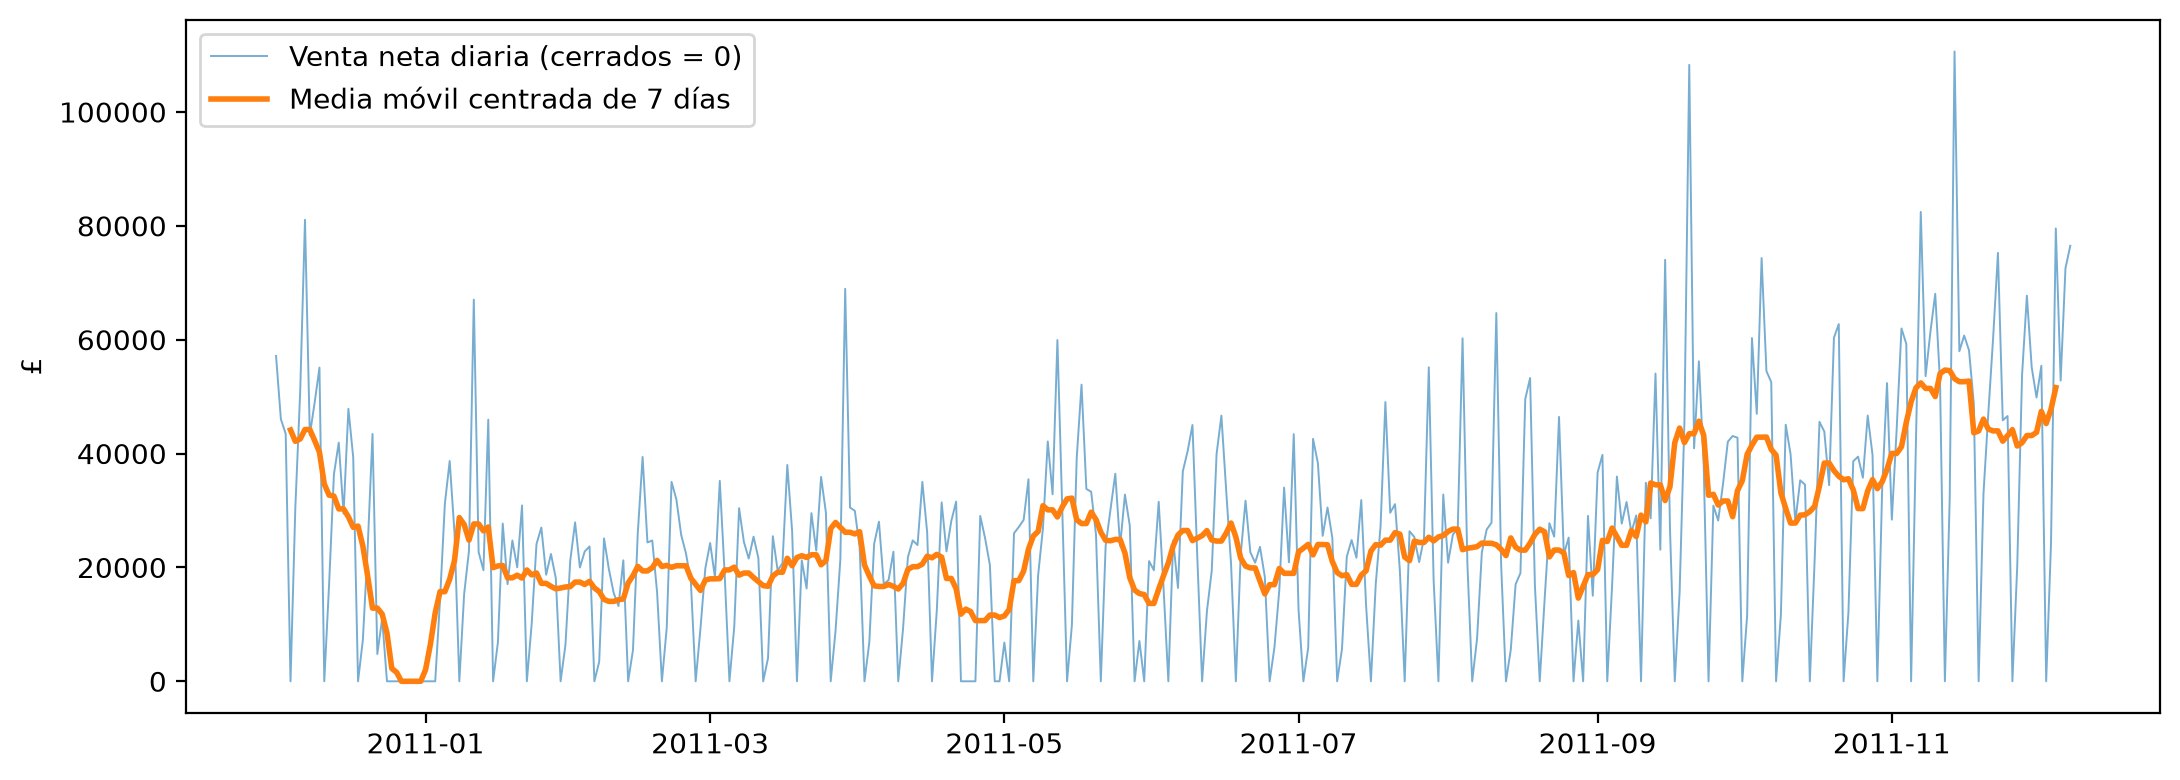
\includegraphics[width=\textwidth]{p3_media_movil.png}
\caption{Venta neta diaria (con los d\'ias cerrados en cero) y su media
m\'ovil centrada de 7 d\'ias. La ca\'ida casi a cero a finales de diciembre de
2010 corresponde al cierre de fin de a\~no.}
\label{fig:ma7}
\end{figure}

Se usa una ventana de 7 d\'ias porque la tienda tiene un ciclo semanal (cierra
los s\'abados y su venta cambia seg\'un el d\'ia): promediar exactamente una
semana completa cancela ese ciclo y deja visible la tendencia. Una ventana de 5
d\'ias no cubrir\'ia el ciclo entero y dejar\'ia parte de la estacionalidad
semanal en la curva; una de 30 d\'ias suavizar\'ia tanto que ocultar\'ia
cambios reales, como la ca\'ida de fin de a\~no o el aumento de
oto\~no. La media es \emph{centrada} para que el valor en el d\'ia $t$ use
los tres d\'ias anteriores y los tres posteriores y quede alineado con la
fecha; una media que solo mira hacia atr\'as desplazar\'ia la tendencia unos
d\'ias hacia el futuro. El costo es que los tres primeros y los tres
\'ultimos d\'ias quedan sin valor.

La tendencia es casi plana de enero a agosto, con una media m\'ovil entre
aproximadamente \pounds 15{,}000 y \pounds 25{,}000 diarios. A partir de
septiembre sube con fuerza y supera los \pounds 50{,}000 en noviembre,
lo que sugiere una estacionalidad anual de fin de a\~no (que con un solo
a\~no de datos no se puede estimar, como se ver\'a en la Parte 5).

\subsection*{3.2 Estacionalidad}

El \'indice estacional de cada d\'ia de la semana es el promedio de
$y_t/\mathrm{MA}_t$ sobre los d\'ias abiertos del entrenamiento (hasta el 30
de septiembre de 2011). La media m\'ovil se calcul\'o solo con datos del
entrenamiento para que los cocientes de los \'ultimos d\'ias no usen
informaci\'on de octubre.

\begin{table}[H]
\centering
\begin{tabular}{l|c}
\hline
D\'ia & \'Indice estacional \\
\hline
Lunes     & 1.1711 \\
Martes    & 1.5479 \\
Mi\'ercoles & 1.2273 \\
Jueves    & 1.5653 \\
Viernes   & 1.1100 \\
Domingo   & 0.5767 \\
\hline
\end{tabular}
\caption{\'Indice estacional por d\'ia de la semana (promedio de
$y_t/\mathrm{MA}_t$). El promedio de los seis \'indices es 1.1997.}
\label{tab:indice}
\end{table}

\begin{figure}[H]
\centering
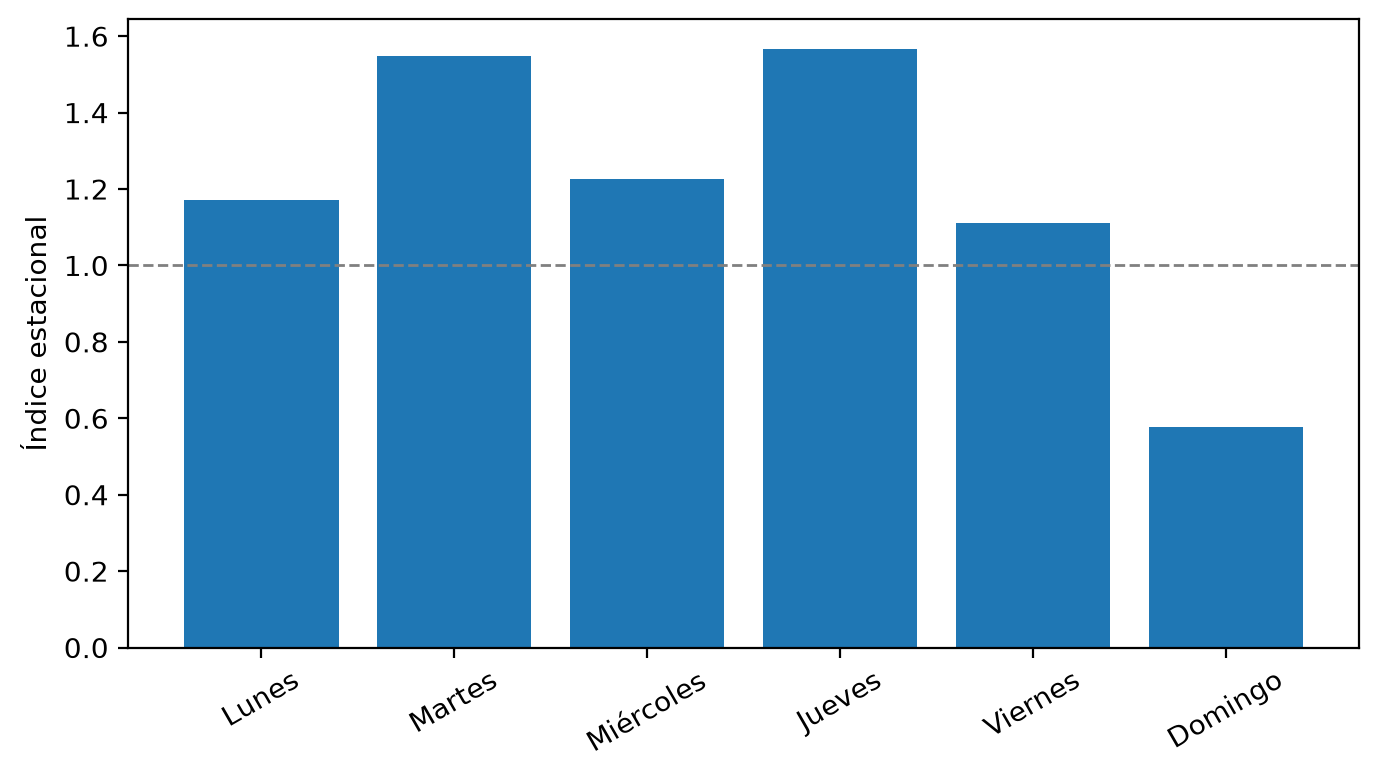
\includegraphics[width=0.7\textwidth]{p3_indice_estacional.png}
\caption{\'Indice estacional por d\'ia de la semana. La l\'inea punteada
marca el valor 1.}
\label{fig:indice}
\end{figure}

Venden m\'as los martes (1.55) y los jueves (1.57), y mucho menos los
domingos (0.58); lunes, mi\'ercoles y viernes quedan intermedios. El promedio
de los seis \'indices no es 1 porque la media m\'ovil divide la venta de la
semana entre 7 d\'ias, incluido el s\'abado cerrado con cero, mientras que los
cocientes se calculan solo en los 6 d\'ias abiertos: si los seis d\'ias
vendieran lo mismo, cada \'indice ser\'ia $7/6\approx1.17$. El valor observado
(1.1997) es algo mayor porque los feriados dentro de la ventana tambi\'en
bajan la media m\'ovil.

\subsection*{3.3 Autocorrelaci\'on}

\begin{figure}[H]
\centering
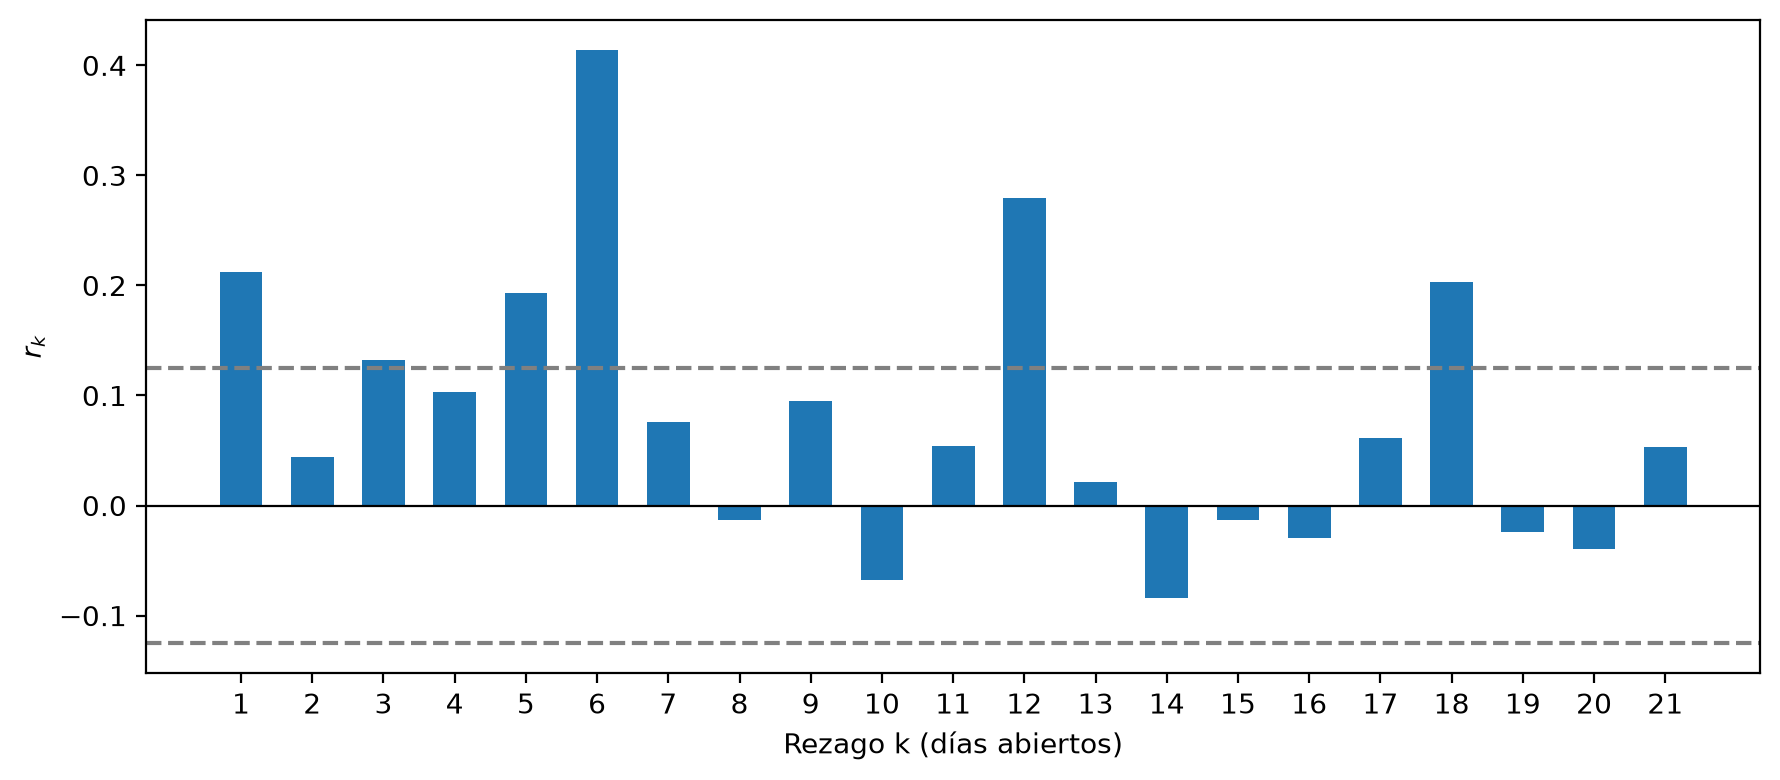
\includegraphics[width=0.85\textwidth]{p3_acf_ventas.png}
\caption{Autocorrelaci\'on muestral $r_k$ de la venta de los d\'ias abiertos del
entrenamiento ($n=245$), con bandas $\pm1.96/\sqrt{n}=\pm0.1252$. Cada rezago
$k$ es un d\'ia abierto, no un d\'ia calendario.}
\label{fig:acf}
\end{figure}

\paragraph{(a)} Seis rezagos se salen de las bandas: 1, 3, 5, 6, 12 y 18. La
serie \textbf{no pasa} la prueba de retardo 1 de la Tarea 2, pues
$r_1=0.212>0.1252$. El pico est\'a en $k=6$ ($r_6=0.414$); como la tienda
abre 6 d\'ias por semana, 6 d\'ias abiertos equivalen a una semana
(unos 7 d\'ias calendario). Los rezagos 12 y 18, tambi\'en altos, son
m\'ultiplos de 6 (2 y 3 semanas). Las pruebas de Ljung--Box rechazan con
claridad el ruido blanco: $Q(6)=71.53$ ($p=1.98\times10^{-13}$) y
$Q(12)=97.57$ ($p=1.66\times10^{-15}$), valores que coinciden con
\texttt{acorr\_ljungbox} de \texttt{statsmodels}.

\paragraph{(b)} Seg\'un la Parte 0, una serie reprueba por dos razones:
memoria y media no constante. Aqu\'i las dos est\'an presentes. El patr\'on de
picos en los m\'ultiplos de 6 es la huella de la media que cambia con el d\'ia
de la semana (el \'indice estacional lo confirma), tal como el patr\'on semanal
de la Parte~0.4 produc\'ia autocorrelaci\'on en el rezago 7 sin memoria
alguna. La tendencia, con una media que sube hacia el final del a\~no, tambi\'en
infla $r_k$ en todos los rezagos. No es posible separar cu\'anto es memoria
verdadera mirando solo esta gr\'afica: eso se hace en la Parte 4, quitando
primero la estacionalidad semanal y revisando qu\'e autocorrelaci\'on queda en
el residuo.

\section*{Parte 4: Del AR(1) al SARIMA}

\subsection*{4.1 Quitar la estacionalidad semanal}

Se ajusta por OLS la venta de los d\'ias abiertos del entrenamiento (245 d\'ias)
contra indicadoras de d\'ia de la semana, sin intercepto. Los coeficientes son
el promedio de venta de cada d\'ia:

\begin{table}[H]
\centering
\begin{tabular}{l|r}
\hline
D\'ia & Coeficiente (\pounds) \\
\hline
Lunes     & 27{,}215.8 \\
Martes    & 35{,}170.0 \\
Mi\'ercoles & 27{,}838.7 \\
Jueves    & 35{,}428.7 \\
Viernes   & 26{,}261.6 \\
Domingo   & 13{,}716.7 \\
\hline
\end{tabular}
\caption{Coeficientes del OLS con indicadoras de d\'ia.}
\label{tab:ols}
\end{table}

\begin{figure}[H]
\centering
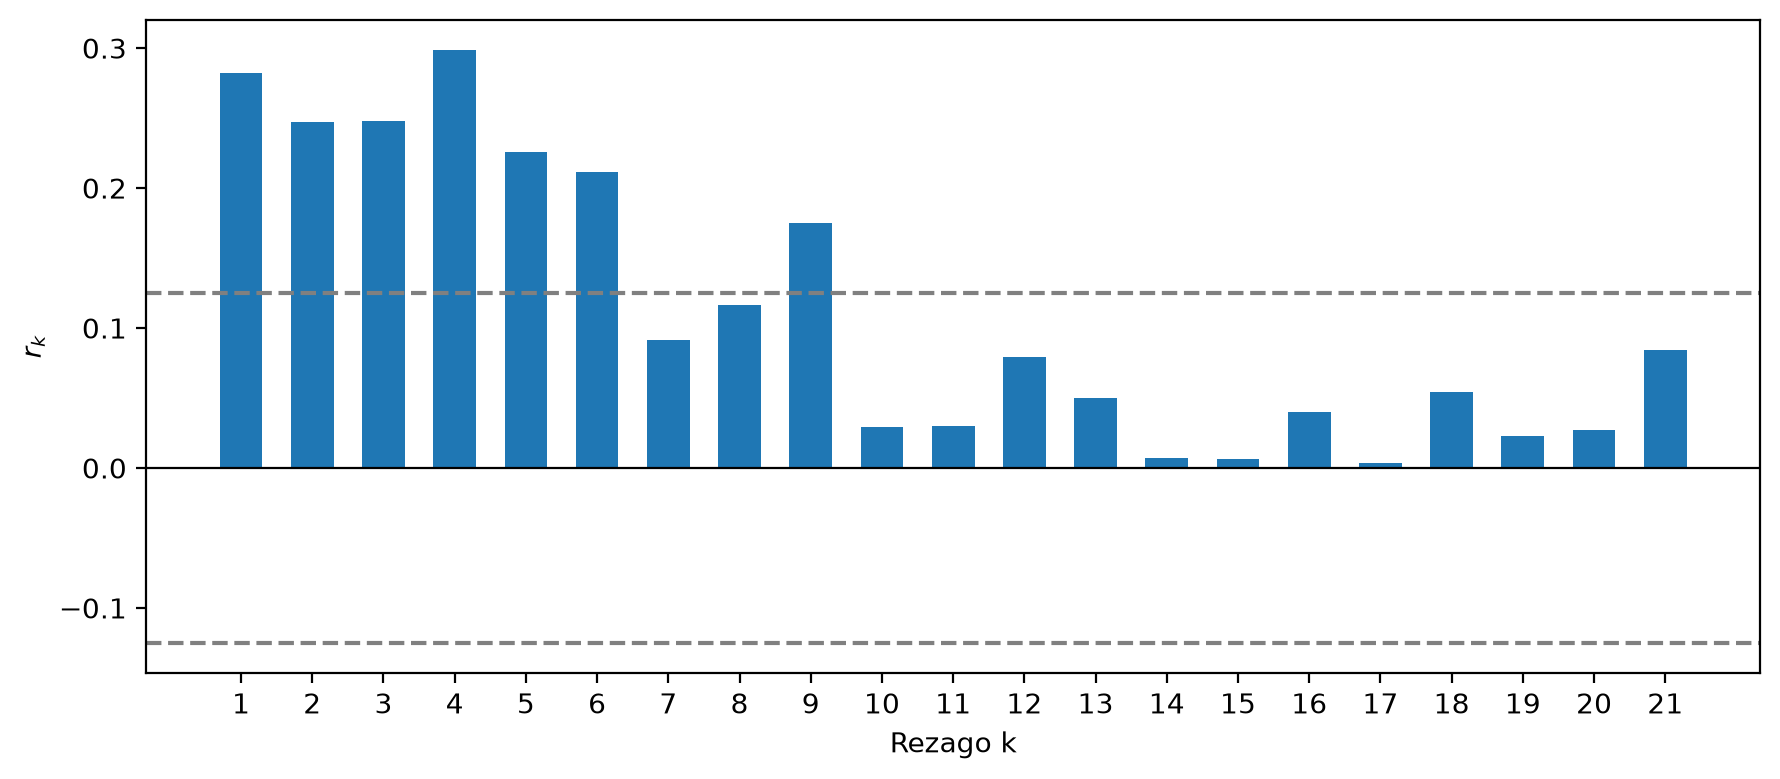
\includegraphics[width=0.85\textwidth]{p4_acf_ols.png}
\caption{ACF de los residuos $e_t$ del modelo con indicadoras de d\'ia, con
bandas $\pm0.1252$.}
\label{fig:acfols}
\end{figure}

Respecto a la ACF de 3.3, los picos de los rezagos 6, 12 y 18 desaparecieron:
el patr\'on semanal ya est\'a fuera. Pero quedan siete rezagos fuera de las
bandas (1 a 6 y 9), todos positivos y similares ($r_1=0.282$, $r_2=0.247$,
$r_3=0.248$, $r_4=0.299$, $r_5=0.225$, $r_6=0.212$), y $Q(6)=96.91$,
$Q(12)=112.43$ ($p\approx10^{-18}$): los residuos no son ruido blanco. La forma
no es la de un AR(1), que decaer\'ia como $\phi^k$ hasta cero, sino la de una
serie que sigue un nivel que cambia lentamente, parecida a la ACF del proceso
con tendencia de la Parte~0. Al modelo le falta capturar ese nivel que se
mueve (la tendencia que se ve en la media m\'ovil de 3.1: baja en invierno y
sube en oto\~no), porque las indicadoras de d\'ia suponen un promedio
constante.

\subsection*{4.2 AR(1) sobre los residuos}

\begin{figure}[H]
\centering
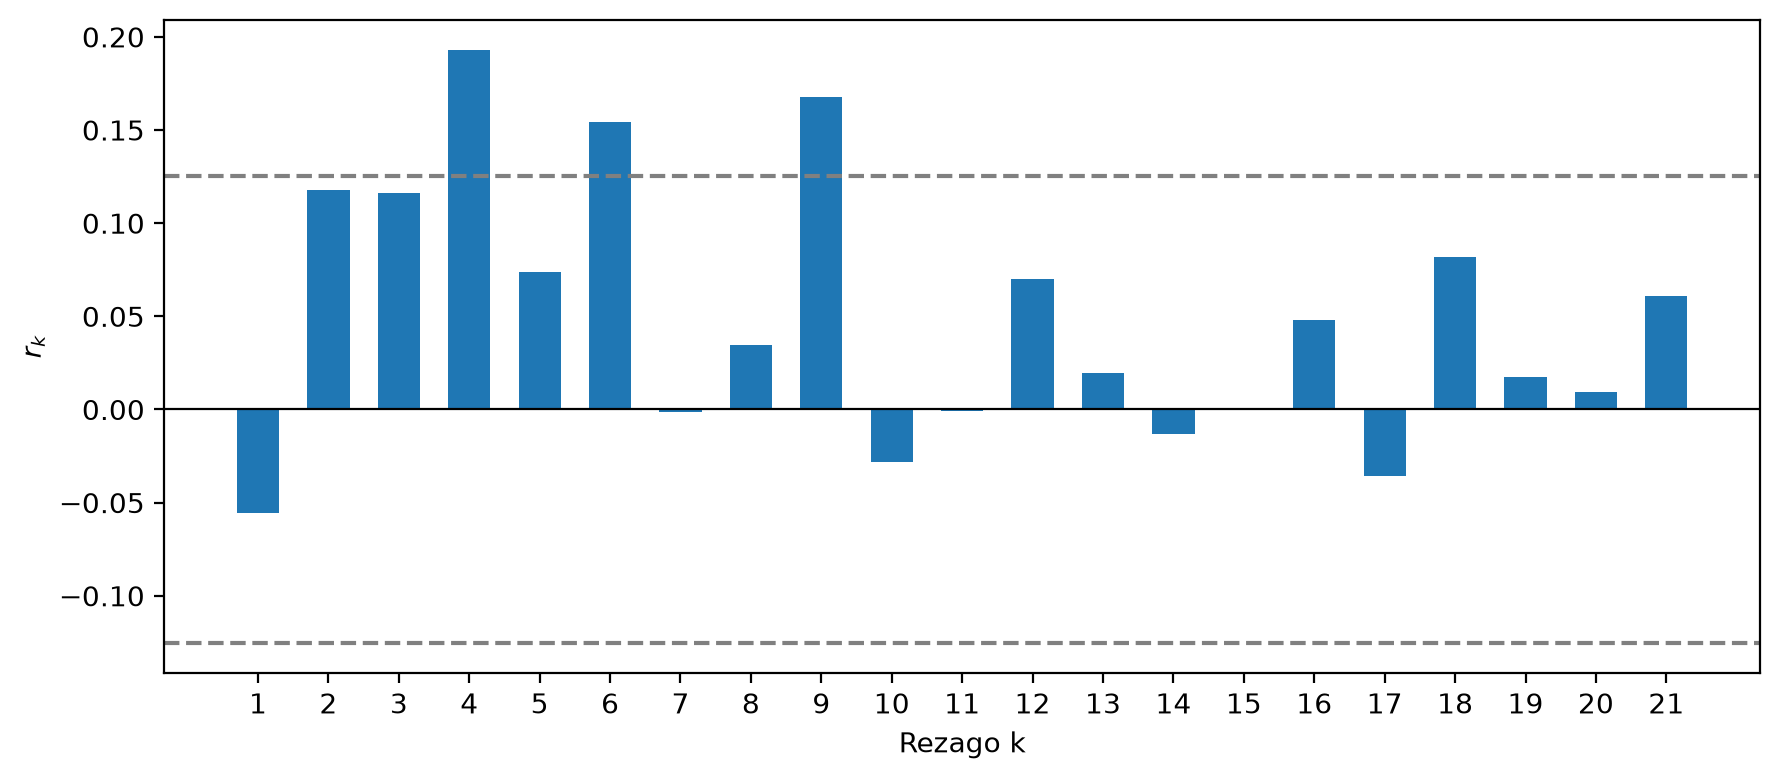
\includegraphics[width=0.85\textwidth]{p4_acf_ar1.png}
\caption{ACF de los residuos $u_t$ del AR(1) ajustado a $e_t$, con bandas
$\pm0.1255$.}
\label{fig:acfar1}
\end{figure}

El OLS de $e_t$ contra $e_{t-1}$ da $\hat c=-100.86$ y $\hat\phi=0.2843$
(e.e.\ $0.0611$). El AR(1) elimina el rezago 1 ($r_1=-0.055$), pero siguen
fuera de las bandas los rezagos 4, 6 y 9, y la prueba de Ljung--Box, con un
grado de libertad menos por haber estimado $\phi$, rechaza: $Q(6)=24.26$
($p=0.000194$, 5 g.l.) y $Q(12)=33.23$ ($p=0.000482$, 11 g.l.). Un AR(1) no
alcanz\'o para lo encontrado en 4.1: la autocorrelaci\'on que queda viene de un
nivel que se mueve lentamente, algo que un AR(1) estacionario con
$\hat\phi=0.28$ no puede reproducir.

\subsection*{4.3 SARIMA}

Se ajustan sobre el logaritmo de la venta diaria de los d\'ias abiertos, con
estacionalidad $s=6$:
\begin{itemize}
\item S1: SARIMA$(1,0,0)(1,0,0)_6$ con constante.
\item S2: SARIMA$(0,1,1)(0,1,1)_6$ sin constante, es decir
$(1-B)(1-B^6)\log y_t=(1+\theta B)(1+\Theta B^6)\varepsilon_t$.
\end{itemize}

\paragraph{Por qu\'e $s=6$ y no 7.} La serie tiene una fila por d\'ia abierto y
la tienda abre 6 d\'ias por semana, as\'i que el mismo d\'ia de la semana se
repite cada 6 filas (lo confirman los picos de $r_k$ en 6, 12 y 18). Se pasa a
\texttt{SARIMAX} el arreglo de valores y no la serie con fechas, porque las
fechas tienen huecos.

\paragraph{D\'onde se rompe esa suposici\'on.} Cuando un feriado cae entre
semana, la fila siguiente no es el d\'ia que corresponder\'ia a la semana
completa de 6 d\'ias abiertos; el ciclo de 6 filas se desfasa. Esto ocurre en
Navidad, Semana Santa y los otros feriados de la Parte~2.

\paragraph{Por qu\'e el logaritmo.} La estacionalidad es multiplicativa (los
\'indices de 3.2 son cocientes) y la variabilidad crece con el nivel de ventas.
El logaritmo convierte los efectos multiplicativos en aditivos y estabiliza la
varianza (FPP2, \S3.2). Para volver a libras se aplica \texttt{exp()} al
pron\'ostico, sin correcci\'on de sesgo.

\paragraph{Convergencia.} S1 no convergi\'o con el n\'umero de iteraciones
por defecto (el indicador de convergencia fue \texttt{False}); al subir
\texttt{maxiter} a 500 s\'i convergi\'o y los par\'ametros cambiaron mucho, as\'i
como la log-verosimilitud, que mejor\'o de $-187.00$ a $-162.47$:

\begin{table}[H]
\centering
\begin{tabular}{l|r|r}
\hline
Par\'ametro de S1 & \texttt{maxiter} por defecto & \texttt{maxiter}=500 \\
\hline
Constante          & 0.8901 & 4.2732 \\
$\hat\phi$ (AR 1)   & 0.1387 & 0.1272 \\
$\hat\Phi$ (AR est.\ 6) & 0.8951 & 0.5165 \\
$\hat\sigma^2$     & 0.2638 & 0.2189 \\
\hline
Log-verosimilitud  & $-187.00$ & $-162.47$ \\
\hline
\end{tabular}
\caption{Par\'ametros de S1 antes y despu\'es de subir \texttt{maxiter}. Se
usa la configuraci\'on que convergi\'o.}
\label{tab:s1}
\end{table}

S2 convergi\'o: $\hat\theta=-0.9092$ (e.e.\ 0.034), $\hat\Theta=-0.6836$ (e.e.\
0.051) y $\hat\sigma^2=0.2139$.

\subsection*{4.4 Diagn\'ostico}

\begin{table}[H]
\centering
\begin{tabular}{l|cc|cc}
\hline
 & $Q(6)$ & $p$ & $Q(12)$ & $p$ \\
\hline
S1 & 9.64 & 0.0469 & 24.73 & 0.00589 \\
S2 & 3.60 & 0.462  &  9.26 & 0.507 \\
\hline
\end{tabular}
\caption{Ljung--Box sobre los residuos, con $m-2$ grados de libertad. En S2 se
descartan los primeros 7 residuos, que son artefactos del arranque de las
diferencias $(1-B)(1-B^6)$.}
\label{tab:diag}
\end{table}

S2 deja residuos de ruido blanco: no se rechaza en ninguno de los dos
rezagos ($p=0.46$ y $0.51$). S1 no: $Q(6)$ rechaza apenas ($p=0.047$) y
$Q(12)$ rechaza con claridad ($p=0.006$), por lo que a S1 le queda
autocorrelaci\'on sin modelar.

\subsection*{4.5 Hacia d\'onde van los pron\'osticos}

S1 es estacionario: como en un AR(1) con $|\phi|<1$, sus pron\'osticos
revierten a la media. A medida que crece el horizonte, el efecto del \'ultimo
dato se desvanece y el pron\'ostico converge a la media incondicional del
logaritmo, $c/((1-\hat\phi)(1-\hat\Phi))\approx10.13$, es decir
aproximadamente \pounds 25{,}000 al aplicar \texttt{exp()}. Este nivel es
coherente con la Parte~3: la media m\'ovil de 3.1 promedia siete d\'ias
calendario, incluido el s\'abado cerrado con cero, as\'i que el nivel de un d\'ia
abierto es unas $7/6$ veces mayor (de \pounds 15{,}000--25{,}000 a
\pounds 17{,}500--29{,}000), y \pounds 25{,}000 cae en ese rango. S1 solo recoge
el nivel medio del entrenamiento y pierde el alza reciente de fin de a\~no.
S2 no es
estacionario: como la caminata aleatoria, no revierte a ninguna media. Su
pron\'ostico conserva el \'ultimo nivel observado junto con el patr\'on
estacional, y su incertidumbre crece sin cota con el horizonte.

\section*{Parte 5: Pronóstico y evaluación}

\subsection*{5.1 Modelos y protocolo}
Sea $y_t$ la venta neta diaria en libras, definida solo en los días abiertos (los días sin ventas son datos faltantes, no ceros). Los días cerrados (sábados y los feriados de la tabla de la Parte 2) se conocen de antemano, por lo que solo se pronostican días abiertos. Se comparan seis modelos:
\begin{itemize}
  \item \textbf{B1 (media histórica):} $\hat y_t=\bar y$, el promedio de todos los días abiertos hasta el origen.
  \item \textbf{B2 (ingenuo estacional):} $\hat y_t$ es la venta del último día abierto con el mismo día de la semana. Si $t-7$ fue día cerrado, se usa el más reciente anterior (por ejemplo, para el 9 de mayo se usa el 18 de abril, porque el 2 de mayo y el 25 de abril fueron feriados).
  \item \textbf{M1 (OLS):} $y_t=\sum_{d}\beta_d D_{d,t}+\gamma\, t+\varepsilon_t$, con indicadores de día de la semana (lunes a viernes y domingo) y tendencia lineal en días calendario.
  \item \textbf{M2 (OLS con rezagos):} $y_t=\sum_d\beta_d D_{d,t}+\phi_1 y_{t-7}+\phi_2 y_{t-14}+\varepsilon_t$, con la misma regla de respaldo de B2 para los rezagos. Las filas sin dos rezagos disponibles se descartan al ajustar.
  \item \textbf{S1:} SARIMA$(1,0,0)(1,0,0)_6$ con constante, sobre $\log y_t$.
  \item \textbf{S2:} SARIMA$(0,1,1)(0,1,1)_6$ sin constante, sobre $\log y_t$.
\end{itemize}
Para S1 y S2 el horizonte $h$ de cada objetivo es su posición entre los días abiertos posteriores al origen, y el pronóstico se transforma con $\exp(\cdot)$ (equivale a la mediana, no a la media). En cada ajuste se verificó \texttt{mle\_retvals["converged"]} con \texttt{maxiter=500}. S1 no convergió con el optimizador por defecto en un único origen (4 de septiembre); con el optimizador \texttt{bfgs} convergió y el pronóstico casi no cambió, por lo que se usó ese reintento (S1: 31 de 32 ajustes convergieron al primer intento y 32 de 32 tras el reintento; S2: 32 de 32).

Las métricas son MAE y RMSE agrupadas sobre todos los días pronosticados.

\textbf{Por qué M2 puede usar $y_{t-7}$ pero no $y_{t-1}$.} El origen es un domingo y los objetivos son los siete días siguientes. Para cualquier objetivo $t$, el día $t-7$ cae a lo sumo en el propio origen, así que $y_{t-7}$ ya se observó. En cambio, $y_{t-1}$ solo se conoce para el lunes (su día anterior es el domingo de origen); para el miércoles, $y_{t-1}$ es el martes, que todavía no ocurrió. S1 sí usa el rezago 1 porque pronostica de forma recursiva: el pronóstico del lunes ocupa el lugar del dato real al pronosticar el martes, y así sucesivamente. Por eso el efecto del último dato observado se desvanece con el horizonte y el pronóstico de S1 revierte a su media (véase 4.5).

\subsection*{5.2 Comparación de esquemas de evaluación}
\begin{itemize}
  \item \textbf{(a) Validación cruzada aleatoria} de 5 pliegues sobre el entrenamiento (hasta el 30 de septiembre), repetida con 10 semillas (2026 a 2035), solo para B1, M1 y M2. Se evalúan 233 días (los 12 primeros se excluyen porque M2 necesita dos rezagos del mismo día de la semana). Se reporta el promedio de las 10 repeticiones. La desviación estándar entre semillas es pequeña (MAE: 36 para B1, 74 para M1 y 105 para M2).
  \item \textbf{(b) Origen móvil semanal en el entrenamiento:} 22 orígenes (domingos del 1 de mayo al 25 de septiembre); cada origen ajusta con datos hasta ese domingo y pronostica de lunes a domingo siguientes, sin evaluar días posteriores al 30 de septiembre (128 días evaluados).
  \item \textbf{(c) Origen móvil en la prueba:} 10 orígenes (domingos del 2 de octubre al 4 de diciembre); el último día evaluado es el 8 de diciembre (58 días). El 9 de diciembre se excluye por estar incompleto.
\end{itemize}

El Cuadro~\ref{tab:p5} resume los resultados.

\begin{table}[H]
\centering
\resizebox{\textwidth}{!}{%
\begin{tabular}{l rr rr rr}
\hline
 & \multicolumn{2}{c}{(a) CV aleatoria} & \multicolumn{2}{c}{(b) Origen móvil, entren.} & \multicolumn{2}{c}{(c) Origen móvil, prueba} \\
Modelo & MAE & RMSE & MAE & RMSE & MAE & RMSE \\
\hline
B1 & 9\,551 $\pm$ 36 & 13\,534 $\pm$ 31 & 10\,228 & 14\,884 & 22\,403 & 26\,927 \\
B2 & --- & --- & 11\,264 & 15\,570 & 14\,147 & 18\,374 \\
M1 & 8\,226 $\pm$ 74 & 11\,336 $\pm$ 88 & 9\,761 & 13\,822 & 15\,176 & 20\,148 \\
M2 & 8\,371 $\pm$ 105 & 11\,772 $\pm$ 118 & 9\,229 & 13\,379 & 15\,156 & 19\,733 \\
S1 & --- & --- & 9\,720 & 13\,737 & 16\,701 & 20\,933 \\
S2 & --- & --- & 10\,031 & 13\,959 & \textbf{12\,356} & \textbf{15\,696} \\
\hline
\end{tabular}}
\caption{Errores de pronóstico diario (\pounds{}) por modelo y esquema de evaluación. En (a) se reporta la media $\pm$ la desviación estándar entre las 10 semillas.}
\label{tab:p5}
\end{table}

\textbf{Por qué (a) no aplica a B2, S1 y S2.} B2 no tiene parámetros que estimar, así que un pliegue de validación no mide nada que un ajuste haya aprendido. S1 y S2 son modelos de series de tiempo que necesitan una serie ordenada y continua: al quitar días al azar quedan huecos y el pronóstico deja de ser un pronóstico hacia adelante condicionado al pasado.

\textbf{Cuál esquema se parece más a (c).} El esquema (b), tanto en procedimiento (solo se usan datos pasados y se pronostica hacia adelante) como en magnitud del error. Para M1 el MAE pasa de \pounds{}8.2k en (a) a \pounds{}9.8k en (b) y \pounds{}15.2k en (c). Pero \textbf{ninguna de las dos se acerca de verdad} a (c): el error de M1 en (b) (\pounds{}9.8k) sigue lejos del de (c) (\pounds{}15.2k), y (b) tampoco ordena igual a los modelos: M2 es el mejor en (b), pero S2 es el mejor en (c), porque en (c) cambió el nivel de las ventas (véase 5.5). Ni (a) ni (b) sirven como estimación confiable del error en la prueba.

\subsection*{5.3 Mejor modelo en la prueba}
S2 es el mejor modelo en la prueba, con MAE de \pounds{}12\,356 y RMSE de \pounds{}15\,696, seguido de B2 (\pounds{}14\,147). La Figura~\ref{fig:p5} muestra los valores reales y los pronósticos de S2, M2 y B2 de octubre a diciembre; las líneas verticales marcan cada origen.

\begin{figure}[H]
\centering
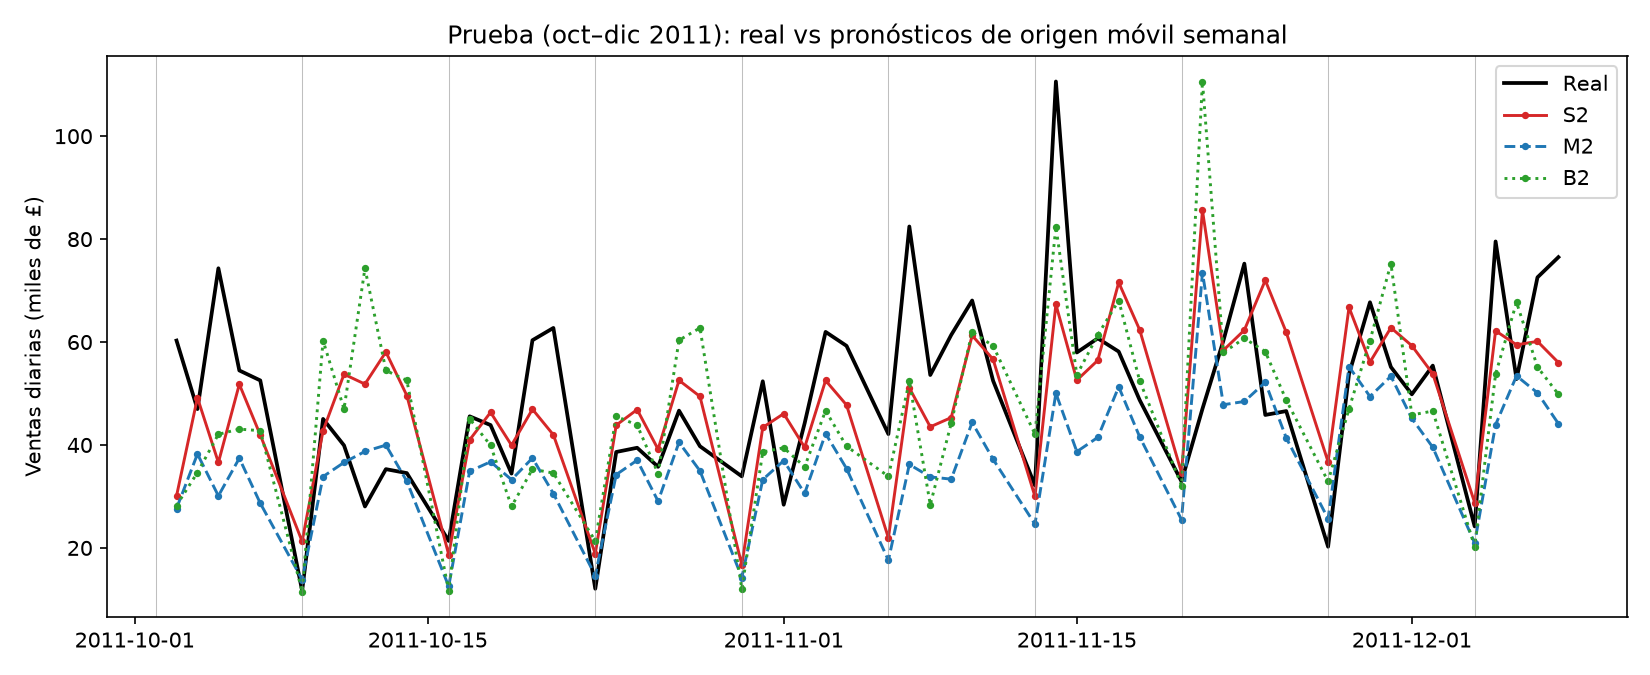
\includegraphics[width=\textwidth]{p5_pronosticos_test.png}
\caption{Ventas reales y pronósticos de origen móvil semanal en la prueba (3 de octubre al 8 de diciembre de 2011).}
\label{fig:p5}
\end{figure}

La causa principal es el sesgo. El Cuadro~\ref{tab:sesgo} muestra el promedio de (real $-$ pronóstico) en la prueba: todos los modelos pronostican por debajo de lo real, pero S2 casi no tiene sesgo, porque al diferenciar su nivel se reajusta al último dato. B1, M1, M2 y S1 se anclan a un nivel promedio (S1 revierte a su media histórica, que es el nivel de aproximadamente \pounds{}25\,000 que se observó en la Parte 4) y subestiman sistemáticamente la subida de octubre a diciembre.

\begin{table}[H]
\centering
\begin{tabular}{lrrrrrr}
\hline
 & B1 & B2 & M1 & M2 & S1 & S2 \\
\hline
Sesgo (real $-$ pron.), \pounds{} & 20\,432 & 2\,736 & 13\,696 & 12\,779 & 14\,235 & 1\,248 \\
\hline
\end{tabular}
\caption{Sesgo medio en la prueba.}
\label{tab:sesgo}
\end{table}

Esto es coherente con la Parte 4, donde S2 tuvo mejores diagnósticos de residuos (Ljung--Box), aunque los residuos limpios por sí solos no garantizan mejor pronóstico: lo que decide en la prueba es que S2 se adapta al nivel.

\subsection*{5.4 La trampa: fuga de información}
Se agregó a M2 la media móvil centrada de 7 días, calculada una sola vez sobre toda la serie. Esta variable es \textbf{ilegal} como predictor: la media centrada de la fecha $t$ promedia $t-3,\dots,t+3$, es decir, incluye el propio valor $y_t$ que se quiere predecir y tres días futuros.

El Cuadro~\ref{tab:trampa} compara M2 con y sin la variable.

\begin{table}[H]
\centering
\begin{tabular}{l rr rr}
\hline
 & \multicolumn{2}{c}{(a) CV aleatoria} & \multicolumn{2}{c}{(b) Origen móvil, entren.} \\
Modelo & MAE & RMSE & MAE & RMSE \\
\hline
M2 & 8\,371 & 11\,772 & 9\,229 & 13\,379 \\
M2 + media móvil centrada & 7\,465 & 10\,051 & 8\,253 & 11\,278 \\
\hline
\end{tabular}
\caption{Efecto de la trampa en (a) y (b).}
\label{tab:trampa}
\end{table}

El error baja cerca de 10\% en ambos esquemas, una mejora aparente que no es real. Que la mejora sea moderada no la hace legítima.

\textbf{Por qué (b) no lo detecta.} El origen móvil solo protege lo que se calcula con datos hasta el origen. Aquí la media móvil se calculó una vez sobre toda la serie, así que para cada día objetivo la columna ya contiene su propio valor y los días posteriores, aunque el modelo ``avance'' semana a semana.

\textbf{Por qué (c) no se puede calcular sin trampa.} En el origen del 4 de diciembre, la media móvil centrada solo es válida hasta el 1 de diciembre (origen menos 3 días). Para pronosticar el 8 de diciembre habría que conocer las ventas hasta el 11 de diciembre, que todavía no han ocurrido. Los datos de octubre y noviembre sí existen en el archivo, y por eso se podría calcular y hacer trampa, pero un pronóstico real no dispone de esos días.

\subsection*{5.5 Origen del error y limitaciones}
\textbf{Esquema frente a cambio de régimen.} Para M1, el paso de \pounds{}8.2k en (a) a \pounds{}9.8k en (b) se debe al esquema: la validación aleatoria usa días futuros para predecir días pasados e interpola, lo que subestima el error. El paso de \pounds{}9.8k a \pounds{}15.2k en (c) se debe sobre todo al cambio de régimen: las ventas de septiembre (\pounds{}1.01M) ya superan las de mayo a agosto (cerca de \pounds{}0.7M al mes), y las de noviembre llegan a \pounds{}1.43M, por lo que una tendencia lineal ajustada al pasado se queda corta (sesgo de \pounds{}13\,696 en la prueba frente a \pounds{}5\,531 en (b)). Una parte del aumento del error absoluto es solo escala: las ventas medias pasan de \pounds{}29.7k en (b) a \pounds{}49.8k en (c), y el error relativo de M1 casi no cambia (33\% en (b) y 31\% en (c)).

\textbf{Qué arregla una mejor validación y qué no.} La causa del esquema (de (a) a (b)) se corrige con un origen móvil que respete el orden del tiempo. La causa del cambio de régimen (de (b) a (c)) no se corrige con ninguna validación interna: un modelo que entrena con meses de ventas moderadas no puede aprender de un pico que todavía no ocurrió. Solo se reduce con más años de historia o con modelos que reajusten su nivel, como S2.

\textbf{Estacionalidad anual con un año de datos.} Con una sola observación por mes, la estacionalidad anual no se puede separar de la tendencia ni del nivel, y los datos empiezan el 1 de diciembre de 2010, por lo que ningún modelo observó un noviembre previo. No se puede saber si el pico de fin de año es un patrón recurrente o un hecho aislado; ningún modelo con un solo año de historia puede anticiparlo.

\section*{Parte 6: Detrás de la serie hay clientes (análisis RFM)}

\subsection*{6.1 Recencia, frecuencia y monto}
Se usan los datos limpios con \texttt{CustomerID} y solo las transacciones anteriores al 1 de octubre de 2011. La recencia $R$ es el número de días entre la última factura de venta del cliente y el 1 de octubre; la frecuencia $F$ es el número de facturas de venta distintas (sin las que empiezan con \texttt{C}); el monto $M$ es la venta neta total del cliente, que incluye sus cancelaciones.

Hay 3\,648 clientes con alguna transacción antes del corte. De ellos, 3\,613 tienen al menos una factura de venta y son la base del análisis; los otros 35 solo tienen cancelaciones, y sin compras no hay recencia, así que quedan fuera. Si alguno de ellos compra después del corte, cuenta como cliente nuevo (6.5).

Siete clientes tienen $M\le 0$ (cuatro con $M=0$ y tres con $M<0$, el menor de $-\pounds{}141.50$): compraron algo y después lo devolvieron por completo o más. No se eliminan, porque el enunciado pide incluirlos en el desempate y porque siguen siendo clientes con una compra y una recencia; el $M$ más bajo los lleva al primer quintil de monto.

No se puede usar nada posterior al 1 de octubre porque el indicador de compra de 6.3 se define con ese periodo. Si $R$, $F$ o $M$ incluyeran compras de octubre a diciembre, quien compró en noviembre tendría una recencia muy pequeña calculada con datos futuros, y el puntaje ``predeciría'' la compra con información que se obtiene después de ella (fuga de información, como en 5.4). Las variables deben construirse con el pasado conocido en el momento de pronosticar.

\subsection*{6.2 Puntajes por quintiles}
Cada dimensión recibe un puntaje de 1 a 5 (en recencia, 5 es el más reciente). Los clientes se ordenan por \texttt{CustomerID}, se barajan con \texttt{numpy.random.default\_rng(2026).permutation} y se aplica \texttt{pd.qcut(rank(method='first'), 5)}.

\textbf{El problema con $F$.} La frecuencia es discreta y muy concentrada: 1\,453 clientes (40\%) tienen $F=1$, más del doble de lo que cabe en un quintil (cerca de 723 clientes, 20\%). Cortar por cuantiles de $F$ directamente falla porque los límites de los grupos se repiten; por eso se ordena por rango y se desempata al azar.

\begin{table}[H]
\centering
\begin{tabular}{c|rr|rr|rr|r}
\hline
 & \multicolumn{2}{c|}{$R$ (días)} & \multicolumn{2}{c|}{$F$ (facturas)} & \multicolumn{2}{c|}{$M$ (\pounds{})} & Clientes \\
Puntaje & mín. & máx. & mín. & máx. & mín. & máx. & \\
\hline
1 & 177 & 304 & 1 & 1 & $-141$ & 224 & 723 \\
2 & 94 & 176 & 1 & 1 & 224 & 412 & 722 \\
3 & 41 & 94 & 1 & 3 & 412 & 788 & 723 \\
4 & 15 & 41 & 3 & 5 & 789 & 1\,693 & 722 \\
5 & 1 & 15 & 5 & 138 & 1\,694 & 202\,084 & 723 \\
\hline
\end{tabular}
\caption{Rango de cada variable por puntaje. Los valores $F=1$, $3$ y $5$ aparecen en más de un puntaje.}
\label{tab:p6rangos}
\end{table}

Dos clientes con la misma $F$ pueden caer en puntajes distintos (por ejemplo, con $F=1$ hay clientes en los puntajes 1, 2 y 3). Esa diferencia no refleja ningún comportamiento: solo depende del orden aleatorio. Por eso el puntaje de $F$ en los niveles bajos es en parte arbitrario, y las diferencias entre puntajes vecinos en ese tramo hay que leerlas con cuidado (véase 6.3).

\subsection*{6.3 ¿Quién compra después?}
Se define $\text{compra}_i=1$ si el cliente tuvo al menos una factura de venta entre el 1 de octubre y el 8 de diciembre. Compraron 1\,835 de los 3\,613 clientes (50.79\%).

\begin{table}[H]
\centering
\begin{tabular}{c|ccc}
\hline
Puntaje & Recencia & Frecuencia & Monto \\
\hline
1 & 0.278 & 0.324 & 0.295 \\
2 & 0.381 & 0.313 & 0.373 \\
3 & 0.553 & 0.458 & 0.458 \\
4 & 0.665 & 0.590 & 0.607 \\
5 & 0.663 & 0.855 & 0.808 \\
\hline
\end{tabular}
\caption{Fracción de clientes que compró entre el 1 de octubre y el 8 de diciembre, por puntaje.}
\label{tab:p6compra}
\end{table}

\begin{figure}[H]
\centering
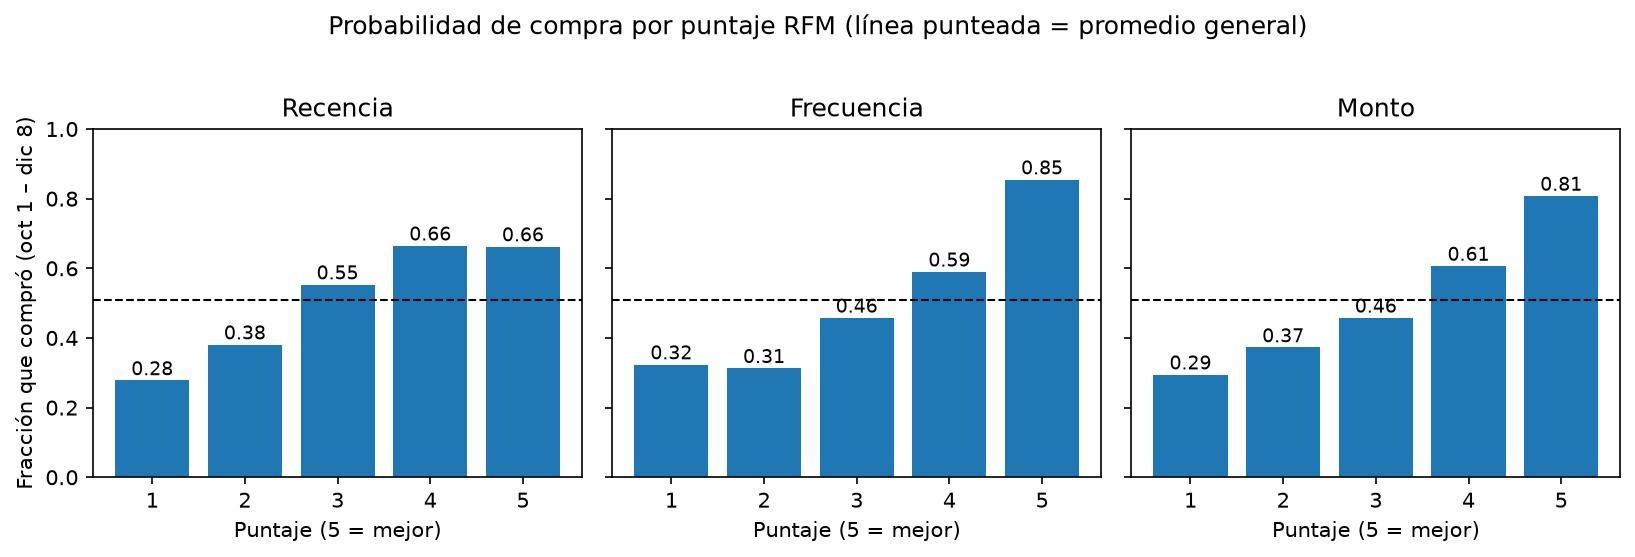
\includegraphics[width=\textwidth]{p6_compra_por_puntaje.png}
\caption{Probabilidad de compra por puntaje de recencia, frecuencia y monto. La línea punteada es el promedio general (50.79\%).}
\label{fig:p6}
\end{figure}

Frecuencia y monto separan mejor que recencia: de 0.32 a 0.85 en $F$ y de 0.29 a 0.81 en $M$, frente a 0.28 a 0.66 en $R$. Las irregularidades de las barras no son sistemáticas: el error estándar de cada fracción es cercano a 0.018, de modo que $R$ en los puntajes 4 y 5 (0.665 y 0.663) y $F$ en los puntajes 1 y 2 (0.324 y 0.313) son prácticamente iguales.

\begin{table}[H]
\centering
\begin{tabular}{l|c}
\hline
Clasificador & AUC \\
\hline
$R$ (signo invertido) & 0.6726 \\
$F$ & 0.7205 \\
$M$ & 0.7089 \\
Suma de los tres puntajes & 0.7342 \\
\hline
\end{tabular}
\caption{AUC de cada dimensión (valores crudos) y de la suma de puntajes como clasificadores de $\text{compra}_i$.}
\label{tab:p6auc}
\end{table}

La mejor dimensión es $F$ (AUC 0.7205). La suma de los tres puntajes solo mejora 0.014 (0.7342) porque las dimensiones se solapan: la correlación de Spearman entre $F$ y $M$ es 0.78, y la de $R$ con $F$ y con $M$ es cercana a $-0.50$. Quien compra mucho suele gastar más y haber comprado hace poco, así que sumar los puntajes aporta sobre todo información repetida.

\subsection*{6.4 Campeones}
Los campeones (puntaje 4 o 5 en las tres dimensiones) son 781 clientes: el 21.62\% de los clientes. Generaron el 53.22\% de la venta neta del 1 de octubre al 8 de diciembre de todos los clientes con \texttt{CustomerID} (\pounds{}2\,396\,663 en total, incluidos los nuevos). Es decir, una quinta parte de los clientes produjo más de la mitad de la venta.

\subsection*{6.5 Clientes nuevos}
Son clientes nuevos los que no tienen ninguna factura de venta antes del 1 de octubre. En la ventana hubo 2\,595 clientes con actividad, de los cuales 723 son nuevos, y ellos generaron \pounds{}378\,213, el 15.78\% de la venta neta.

\begin{table}[H]
\centering
\begin{tabular}{l|rr}
\hline
Grupo & Clientes & Fracción de la venta (oct--dic 8) \\
\hline
Campeones & 781 & 53.22\% \\
Con RFM, no campeones & 2\,832 & 31.00\% \\
Nuevos (sin venta antes del 1 de oct.) & 723 & 15.78\% \\
\hline
\end{tabular}
\caption{Reparto de la venta neta del 1 de octubre al 8 de diciembre (\pounds{}2\,396\,663) entre los tipos de cliente.}
\label{tab:p6resumen}
\end{table}

Un análisis RFM, o cualquier modelo construido cliente por cliente, \textbf{no puede pronosticar esa venta}: sus variables salen del historial del cliente, y un cliente nuevo no tiene historial. Un pronóstico bottom-up (se pronostica a cada cliente y se suman) solo suma clientes que ya existen, así que subestimaría la venta total en una fracción cercana a la de los nuevos (15.78\% en esta ventana) salvo que se le agregue un modelo aparte de captación. Además, la serie diaria de la Parte 5 incluye ventas sin \texttt{CustomerID}, que tampoco ve ningún análisis cliente por cliente.

El pronóstico top-down de la Parte 5 sí ``ve'' a los clientes nuevos, aunque no los identifique: modela el total, y el total ya contiene el flujo habitual de clientes nuevos. En la prueba, S2 tuvo un sesgo de solo \pounds{}1\,248 (cerca del 2.5\% de la venta media), mientras que ignorar a los nuevos habría dejado fuera cerca del 16\%. Esto vale mientras la captación de clientes se parezca a la pasada. Lo mismo ocurre con las recomendaciones del Proyecto~1 (dónde invertir presupuesto de marketing): parten de hogares ya observados y no dicen cuánto vale atraer hogares que todavía no compran.

\section*{Uso de herramientas de IA}
Se usó Claude (Anthropic) como asistente a lo largo de toda la tarea, trabajando por partes en una conversación continua. El reparto fue el siguiente.
\begin{itemize}
  \item \textbf{Lo que hizo Claude:} propuso la estructura del repositorio y del notebook; escribió borradores del código de cada parte (simulaciones, \texttt{limpiar}, descomposición, SARIMA, origen móvil, RFM); redactó borradores del documento en \LaTeX{}; y revisó las respuestas del autor, señalando errores e imprecisiones. También repitió los cálculos por su cuenta con los mismos datos para comprobar que coincidieran con los del notebook (por ejemplo, la limpieza, de 541{,}909 a 531{,}223 filas, y los resultados de las Partes 4, 5 y 6).
  \item \textbf{Lo que hizo el autor:} ejecutó todo el código en su propio notebook y comparó cada resultado, tomó las decisiones de limpieza de la Parte 1 a partir de su exploración de los datos, escribió y corrigió las respuestas de análisis, y revisó el documento final.
\end{itemize}
 
\paragraph{Ejemplos de cómo se trabajó.}
\begin{enumerate}
  \item \textbf{Parte 0.4(b).} El autor anticipó que el patrón semanal casi no se rechazaría al 5\% y que la autocorrelación sería alta. Claude lo comprobó por simulación (rechazo cercano a 10.5\% y $\bar r_7\approx0.26$) y el autor corrigió su explicación.
  \item \textbf{Parte 1.4.} Al revisar las seis líneas de mayor valor se vio que eliminar los \texttt{StockCode} que no son producto dejaba una venta de \pounds{}38\,970 sin su cancelación (\texttt{C556445}); de ahí salió la regla (c) de la bitácora.
  \item \textbf{Partes 5 y 6.} Claude contrastó las explicaciones del autor con los datos y corrigió afirmaciones: el aumento del error en la prueba no se debía a mayor volatilidad (el error relativo casi no cambia, sino el nivel de ventas), y las tres dimensiones del RFM no están todas altamente correlacionadas ($R$ lo está solo de forma moderada).
  \item \textbf{Revisión del documento.} Claude compiló el archivo \texttt{.tex} y detectó una referencia fija a una tabla con el número equivocado y diferencias de numeración, que se corrigieron.
\end{enumerate}
  
Los resultados numéricos provienen del notebook del repositorio y fueron revisados por el autor.
 
\end{document}
\end{document}